
\documentclass[14pt]{extarticle}
\usepackage{graphicx}
\usepackage{pdfpages}
\usepackage[T1]{fontenc}
\usepackage[margin=1in]{geometry}

\graphicspath{ {./images/} }

\begin{document}
    \pagenumbering{arabic}
    \pagestyle{plain}

    \title{\Huge Assignment 3\\ Computer Networks}
    \author{\huge Vikas Gola : 2016UCS0023}
    \maketitle
    \newpage

    \noindent
    \textbf{\large Question 1}
    Enumerate the steps and briefly discuss how the utility traceroute works using an illustrative website as
the argument to it. In your explanation of the tool operation discuss the answers to following questions
w. r. to traceroute
    \begin{itemize}
        \item What if there was no TTL field in the invocation of the traceroute at all?
        \item How will the routers in between determine whether the TTL value limit has reached ?
        \item Should an intermediate router that receives a traceroute packet always respond with an ICMP TTL
        exceeded message ? If the answer is a yes, reason why and if the answer is a no, then argue how do
        we know the address of all the routers/hops in between us and the destination ?
        \item Why does traceroute make use of a destination UDP port number which is invalid - i.e. it sends a
        packet to a UDP port in the range 33434 to 33534 ?
        \item How do we know the address of all the routers/hops in between us and the destination when using
        the traceroute?
        \item How is traceroute latency calculated?
    \end{itemize}
    \textbf{\large Answer}
    Traceroute is a network diagnostic tool to examine the path taken by the packets from your computer to destination to determine the problems in network.
    Traceroute uses TTL which stands for Time To Live which is in IP packet, TTL is used to prevent the Loop in a network, When IP packet forward from one router to another, It decrements the TTL Value by one, When the TTL value will be Zero, The packet will be discarded.
    \begin{itemize}
        \item If there was no TTL field in the invocation of the traceroute at all, the packet will run and go forever or can say flow endlessly from one router to another and goes forever searching for the destination machine. 
        \item TTL limit is set by the sending host in header of packet which is 8 digit binary field which is decreased by the all router and checked if limit has been reached or not. 
        \item No, sometimes routers set "time exceeded" message to that which has been killed and in that case no information return and we don't able to identify.
        \item Traceroute make use of destination UDP port number which is invalid so that it can know that final destination has been reached by getting the message "ICMP Destination/PORT Unreachable". 
        \item Traceroute sends the packet with starting TTL 1, 2 , 3 and so on till we don't reach the final destination. Each time traceroute send the packet it gets the "ICMP TTL exceeded messages" by that router which contains the IP of that router and hence it get to know the IP's.
        \item the route is recorded as the round-trip times of the packets received from each successive host (remote node) in the route  the sum of the mean times in each hop is a measure of the total time spent to establish the connection.
    \end{itemize}
    \vspace{1cm}

    
    \textbf{\large Question 2}
    Execute the traceroute command with www/yahoo.com as argument. Write down the IP address of
yahoo.com that was used for the trace route. Determine the number of iterations required to determine
route. Enlist the IP addresses of all the machines between the source and the destination. What is the
average round trip time of the packet that reached the destination ?\\[10pt]
    \textbf{\large Answer}
    IP address of the www.yahoo.com is 98.137.246.8. 22 iterations are required to determine the route. IP address of the all machines \\[8pt]
    The average round trip time of the packet that reached the destination is 328.25.
    \begin{itemize}
        \item 10.10.50.1
        \item 10.10.10.10
        \item 10.119.231.165
        \item 10.148.6.81
        \item 10.255.238.69
        \item 10.255.238.189
        \item 10.152.7.38
        \item 115.248.54.102
        \item * * *
        \item 62.216.147.73
        \item 85.95.26.233
        \item 85.95.26.241
        \item 195.66.224.129
        \item 216.115.100.26
        \item 216.115.104.120
        \item 184.165.16.44
        \item 216.115.96.34
        \item 216.115.96.204
        \item 66.196.67.109
        \item 67.195.37.97
        \item 98.137.120.6
        \item 98.137.246.8
    \end{itemize} 
    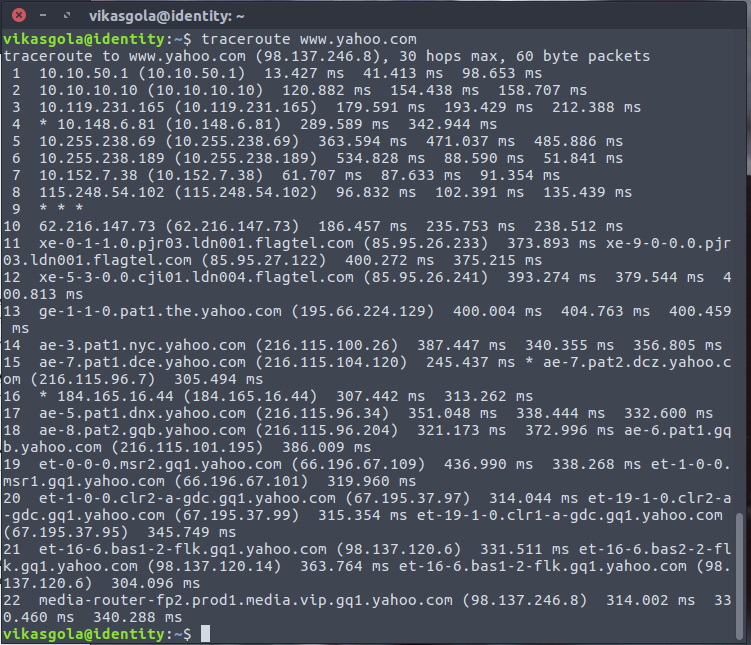
\includegraphics[scale=0.48]{2}
    \vspace{1cm}


    \noindent
    \textbf{\large Question 3}
    With respect to the question no 2, run traceroute on one window of your OS and run tcpdump on the
    other window. Analyze the output of tcpdump. Answer the following questionsm giving appropriate
    hihglighted snapshots in support of your answer :
    \begin{itemize}
        \item How many packets are send by traceroute in each iteration ? How can you prove this using the
        tcpdump output.
        \item Consider one specific iteration of traceroute invocation/iteration. For this specific iteration, what
        are the individual round trip times of each of the three probes sent ? What is the average round
        trip time ? Does it match with the round trip time returned by traceroute ?
        \item In each iteration of traceroute does it use the same port number for the destination ? IF yes, reason
        why and if no, then also argue why does it do so.
    \end{itemize}
    \textbf{\large Answer}
    \begin{itemize}
        \item 3 packets are send by traceroute in each iteration because tcpdump output shows three packets to same IPA.
        \item For first iteration 5.18 , 5.16 and 5.22 are the round trip times for each three probes sent.
        \item NO, it don't use same port number for destination in the each iteration.
    \end{itemize}
    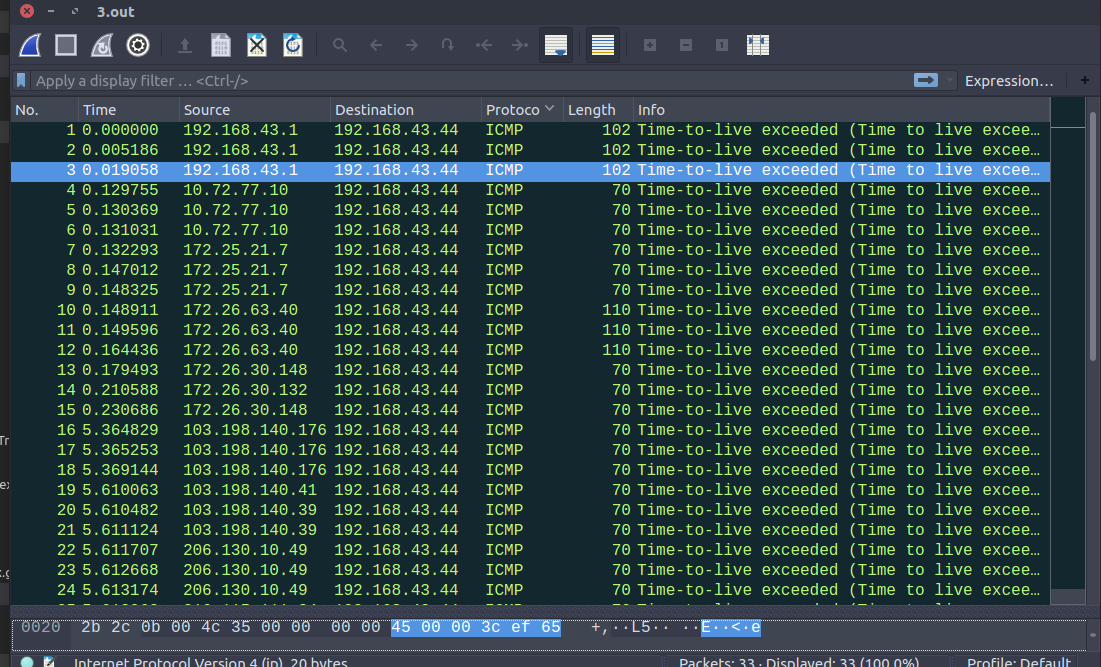
\includegraphics[scale=0.3]{3_0}
    \\[10pt]
    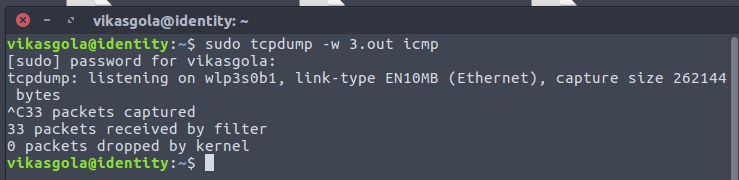
\includegraphics[scale=0.6]{3_1}
    \\[10pt]
    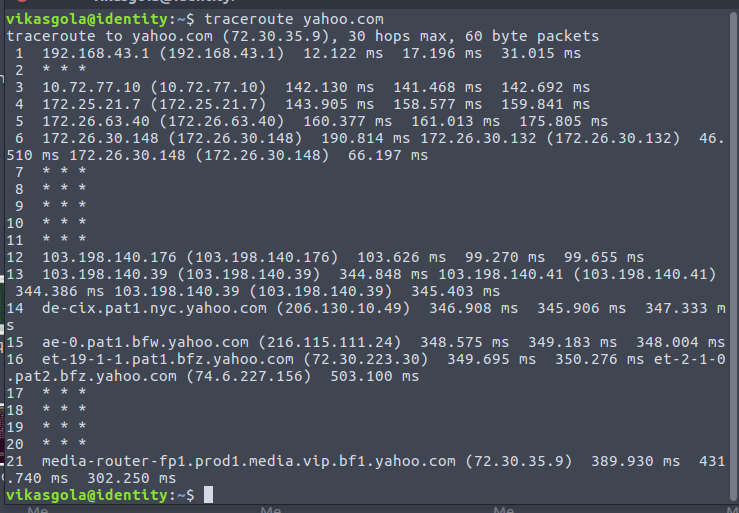
\includegraphics[scale=0.6]{3_2}\\
    \vspace{1cm}


    \noindent
    \textbf{\large Question 4}
    Use the Visual traceroute command at https://www.monitis.com/traceroute/. What is the source ad-
    dressand the destination address of these packets ?\\[10pt]
    \textbf{\large Answer}\\
    Source address = 10.0.0.0\\
    Destination address = 98.138.219.231\\[10pt]
    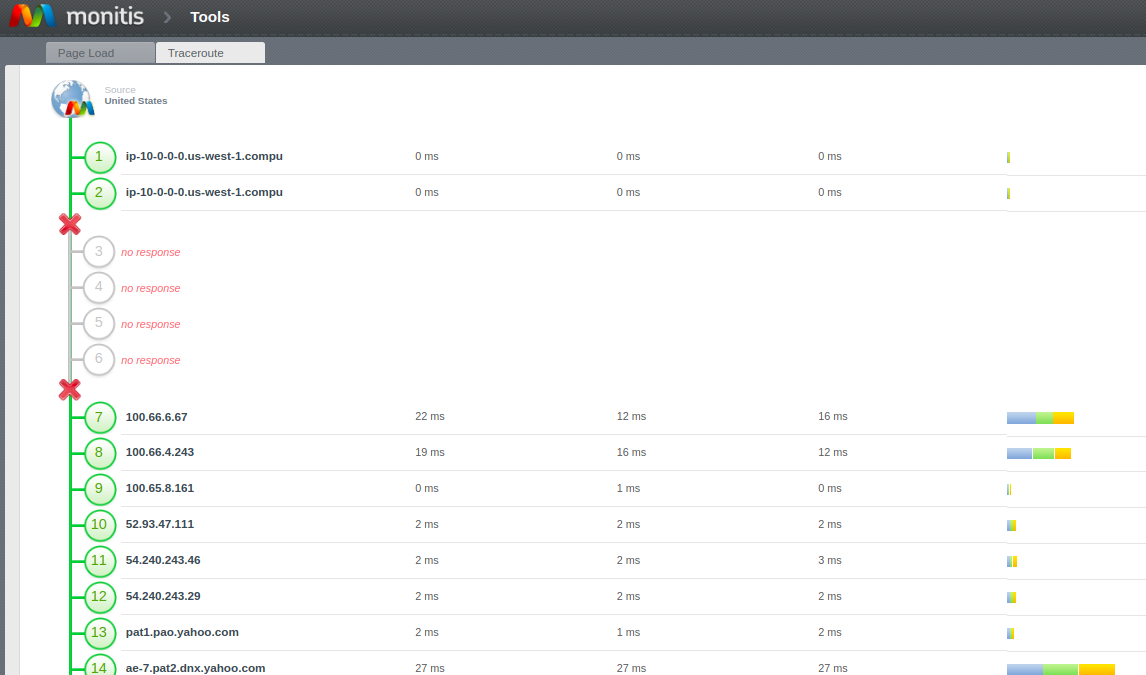
\includegraphics[scale=0.4]{4-1}
    \\[10pt]
    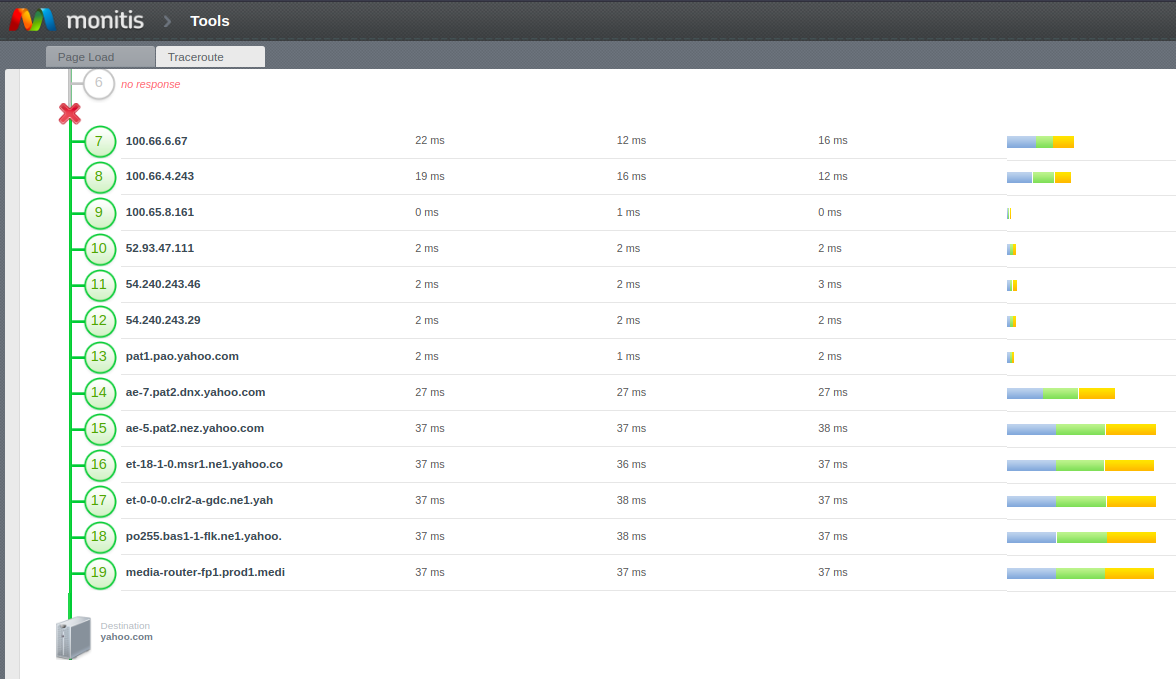
\includegraphics[scale=0.4]{4-2}
    \vspace{1cm}

    \noindent
    \textbf{\large Question 5}
    If you think a firewall stopped the packet, how can one know that a firewall has come in the way ? What
do you think the IP address of that firewall is based on where the trace route stopped?\\[10pt]
    \textbf{\large Answer}
    If traceroute is not able to determine the path between the source and destination then it is firewall which is dropping these packets and not able to detect the path.
    Here is the example where traceroute indicates that there is firewall present in path.
    \\
    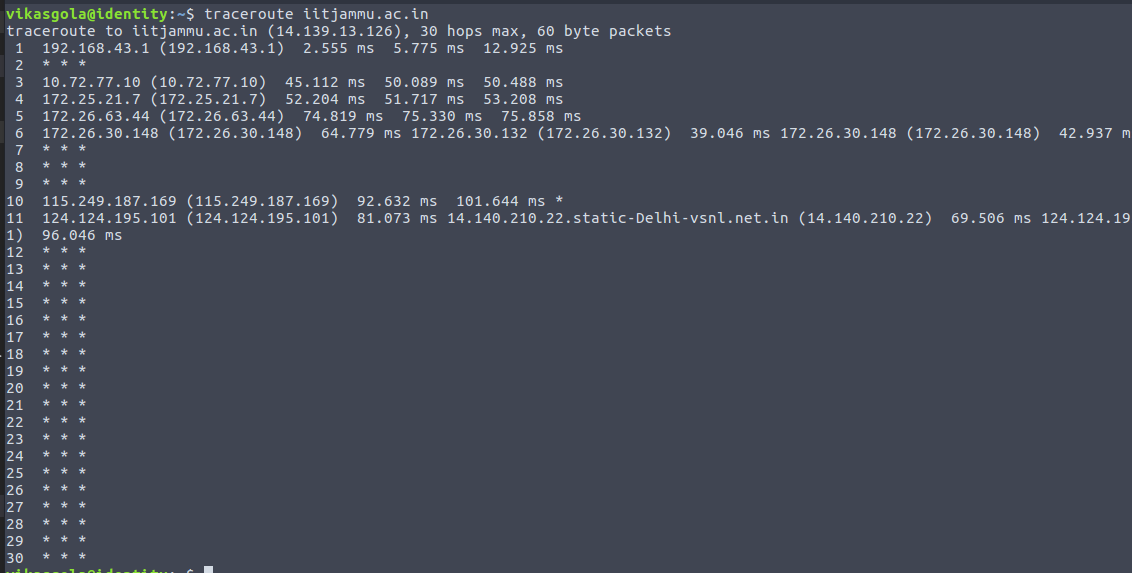
\includegraphics[scale=0.4]{5}
    \vspace{1cm}

    \noindent
    \textbf{\large Question 6}
    If a firewall stopped has not obstructed the packet sent, what does the last IP address appearing in the
trace route list indicate ?\\[10pt]
    \textbf{\large Answer}
    The last address in traceroute list is the destination IP address if no firewall has stopped the sent packet.
    \vspace{1cm}

    \noindent
    \textbf{\large Question 7}
    Enlist and briefly explain all the usages of the ping program - explain each use with the help of an
    example.\\[10pt]
    \textbf{\large Answer}
    \begin{itemize}
        \item \textbf{Host is Up or Not}\\
        ping can be used to check if host is live or not.
        \\
        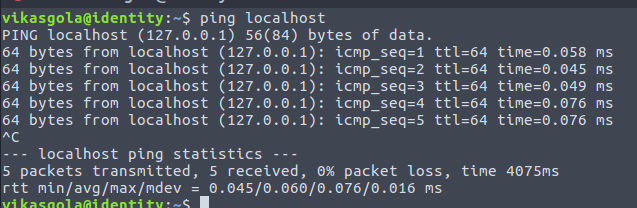
\includegraphics[scale=0.5]{7_1}
        \item \textbf{Destination IP}\\
        ping is also used to find the destination IP address.
        \\
        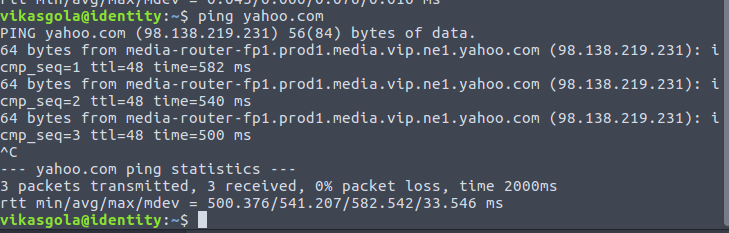
\includegraphics[scale=0.5]{7_2}
        \item \textbf{As traceroute}\\
        ping can also be use alternative to traceroute to find the ip address of the middle routers in the path or to find the path between source and destination.
        \\screenshot is included in next question where we have used ping as traceroute.
        \item \textbf{Check whether the local network interface is up and running}
        ping is also use to check if the local network interface is up and running or not.\\
        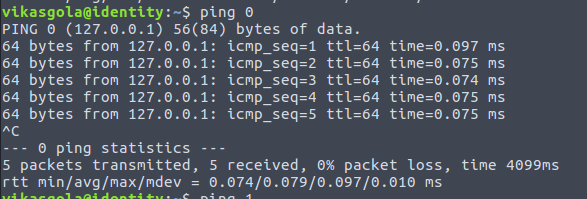
\includegraphics[scale=0.5]{7_3}
        \item \textbf{Flood the network}\\
        ping is also use to send large number of packets to host.\\
        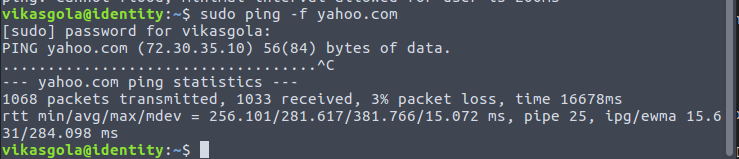
\includegraphics[scale=0.5]{7_4}
        \item \textbf{Record and print route of how ECHO\_REQUEST sent and ECHO\_REPLY received}
        It records, and prints the network route through which the packet is sent and received.
    \end{itemize}
    \vspace{1cm}

    \noindent
    \textbf{\large Question 8}
    Write a small shell script that uses ping to simulate the working of traceroute. Briefly explain the
    operation of the script.\\[10pt]
    \textbf{\large Answer}\\
    \indent
    \textmd{for i in {1..30};do\\
    \indent
    ping -t \$i -c 1 yahoo.com;\\
    \indent
    done
    \indent | grep "Time to live"}\\
    This script contains a for loop which runs 30 times and pings the destination address with TTLs 1 to 30 one by one. grep command help to capture only the required TTL reply and shows.\\[10pt]
    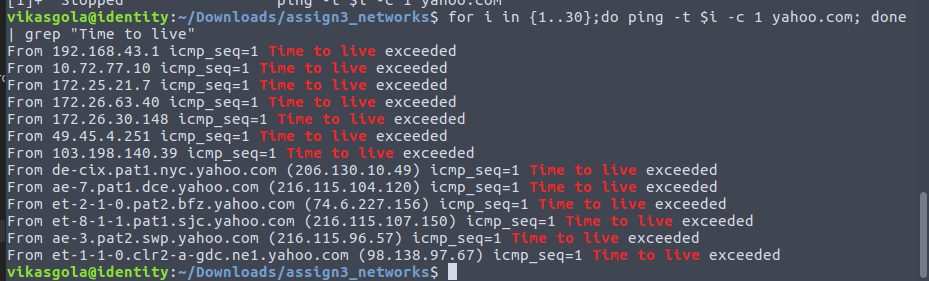
\includegraphics[scale=0.5]{8}
    \vspace{1cm}

    \noindent
    \textbf{\large Question 9}
    Explain all the approaches that can be used to do a ping sweep.\\[10pt]
    \textbf{\large Answer}
    There are number of commands to do ping sweep which are gping, fping and nmap. Usually ping sweep contains the ICMP ECHO request but we can also use ICMP timestamp and ARP for the same work.
    \vspace{1cm}
    
\end{document}